   
\documentclass[11pt]{article}
\renewcommand{\baselinestretch}{1.05}
\usepackage{amsmath,amsthm,verbatim,amssymb,amsfonts,amscd, graphicx}
\usepackage{subcaption}
\graphicspath{{./plot/}}
\topmargin0.0cm
\headheight0.0cm
\headsep0.0cm
\oddsidemargin0.0cm
\textheight23.0cm
\textwidth16.5cm
\footskip1.0cm
\theoremstyle{plain}

 \begin{document}
 



\title{Homework 5 Machine Learning}
\date{}
\author{Marco Treglia}
\maketitle

\section{Clustering }
Clustering is a technique for finding similarity groups in a data, called clusters. It attempts to group individuals in a population together by similarity, but not driven by a specific purpose. Clustering is often called an unsupervised learning, as you don’t have prescribed labels in the data and no class values denoting a priori grouping of the data instances are given.  The goal is to assign a cluster to each data point.
\\
\subsection{K-Means}
 K-means is a clustering method that aims to find the positions $\mu _{i}\; \; ,\; i\; =\; 1\; ...\; k\;  $ centroid of the clusters that minimize the distance from the data points to the cluster. K-means clustering solves:

$$ \arg \; \min _{c}\; \sum_{i=1}^{k}{\sum_{x\; \in \; c_{i}}^{}{d\left( x,\; \mu  \right)\; =\; }}\arg \; \min _{c}\; \sum_{i=1}^{k}{\sum_{x\; \in \; c_{i}}^{}{\left| \left| x\; -\; \mu  \right| \right|^{2}}}\;  $$  
 \\
 with $c_{i}^{}$ et of points that belong to cluster $i$
 \\
 \subsection*{Algorithm}

1) Initialize the center of the clusters : 
$$\mu _{i} = some value \; \; ,\; i\; =\; 1\; ...\; k\;  $$
2) Attribute the closest cluster to each data point : 
$$c_{i}\; =\; \left\{ j\; :\; d\left( x_{j}\; ,\; \mu _{i} \right)\; \leq \; d\left( x_{j}\; ,\; \mu _{k} \right)\; ,\; k\; \neq \; i\; ,\; j\; =\; 1,\; .\; .\; .,\; n \right\}$$
3) Set the position of each cluster to the mean of all data points belonging to that cluster:
$$ \mu _{i}\; =\; \frac{1}{\left| c_{i} \right|}\sum_{j\; \in \; c_{i}}^{}{\; x_{j}\; ,\;\forall i\; } $$
4) Repeat steps 2-3 until convergence.
\newpage
\subsection{Gaussian Mixture Model  (GMM)}
GMM A Gaussian Mixture Model (GMM) is an extension of the K-means model , wich cluster are modolled with gaussian distribuition.  So we have not ony their mean but also the covariance that describe their ellipsoidal shape , then we can fit the model by maximizing the likelihood of the observed data. This estimation is given by using the iterative Expectation-Maximization (EM), that will assign data to each cluster with some soft probability. 

 
 
 
 
 \subsection{Visualization Clustering}
 \subsection*{K-Means}
 
 
\begin{center}
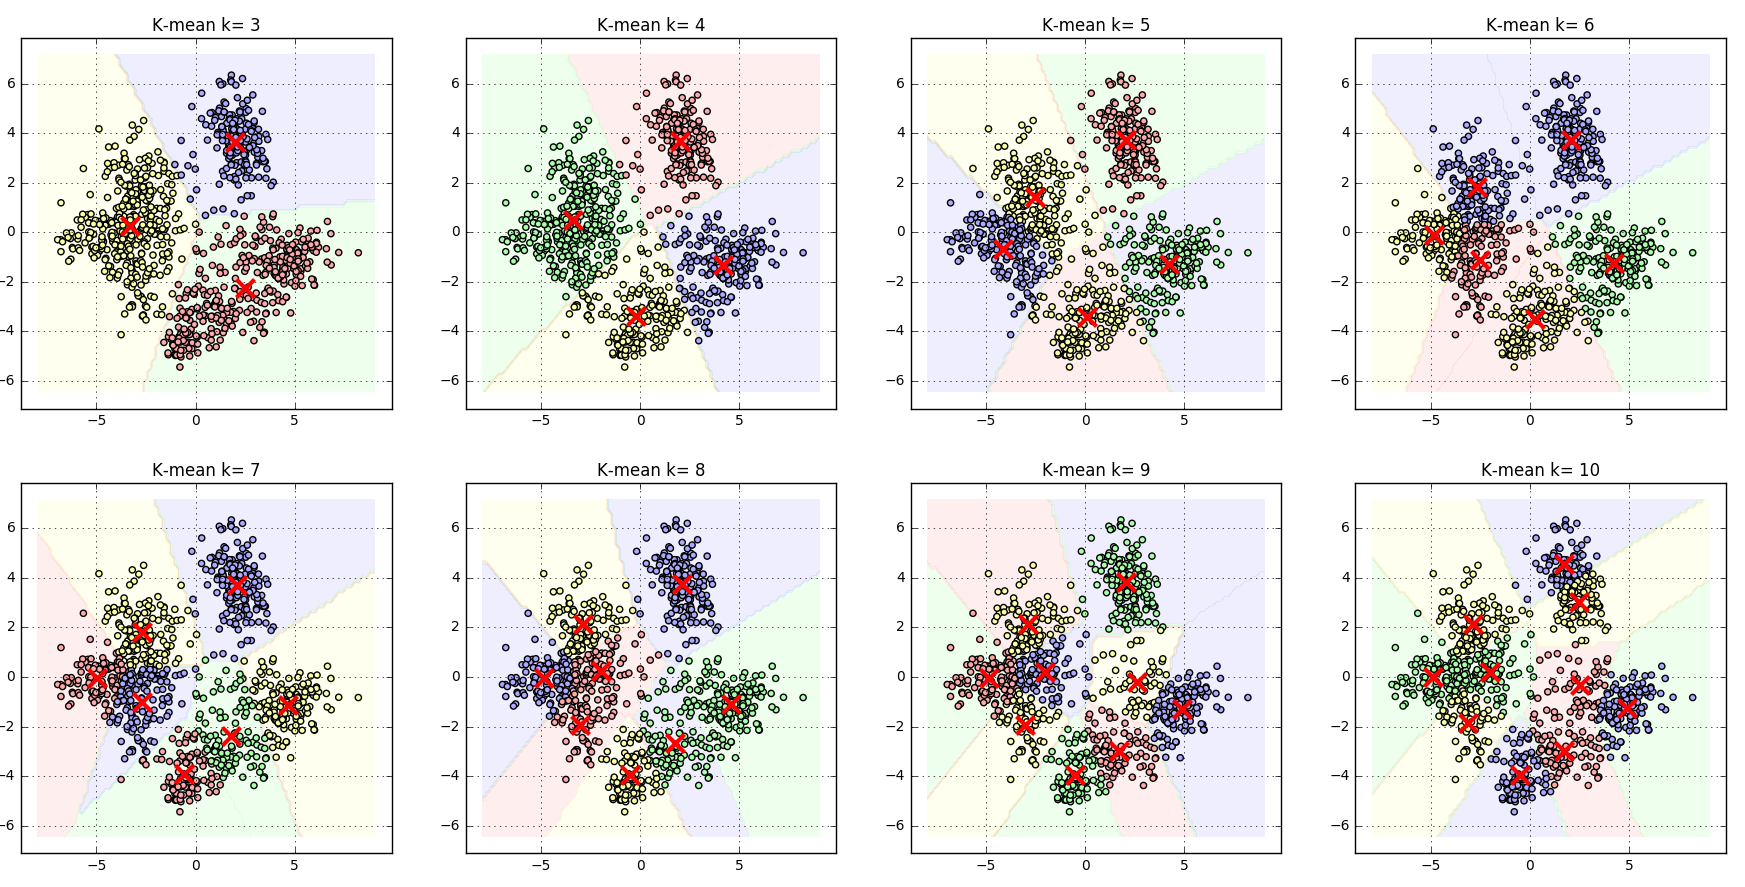
\includegraphics[scale=0.28]{1}
\end{center}

Here the result of clissified our data with K-means from 3 to 10 cluster.
\\
\\
\begin{center}
\begin{tabular}{|r |r |r |r |}

\hline
   K &   Normalized mutual &   Homogeneity &   Purity \\
\hline
   3 &            0.625751 &      0.50771  & 0.584906 \\
   4 &            0.718065 &      0.656366 & 0.748058 \\
   5 &            0.712958 &      0.712744 & 0.863485 \\
   6 &            0.679237 &      0.713051 & 0.842397 \\
   7 &            0.659002 &      0.720104 & 0.834628 \\
   8 &            0.658886 &      0.740584 & 0.843507 \\
   9 &            0.649282 &      0.748835 & 0.833518 \\
  10 &            0.635634 &      0.755502 & 0.835738 \\
\hline
\end{tabular}
 \end{center}
 
 
 
 \begin{center}
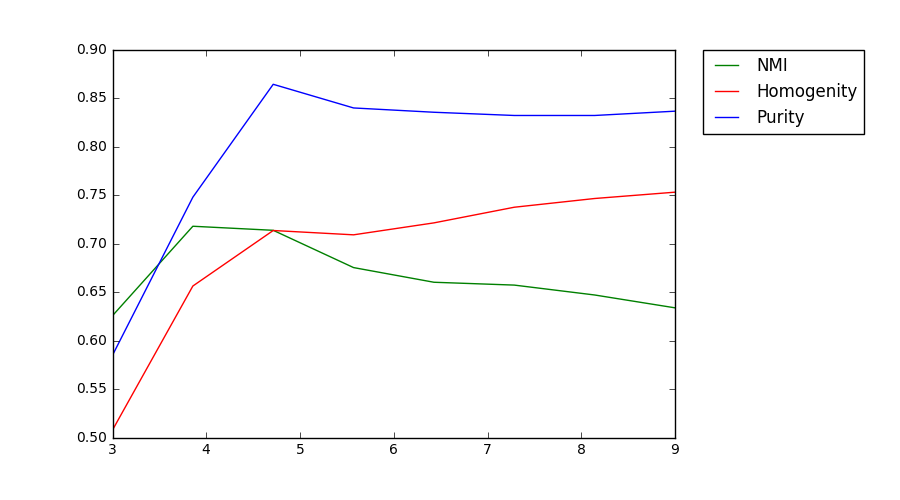
\includegraphics[scale=0.50]{2}
\end{center}
 
\subsection*{GMM}
 
 \begin{center}
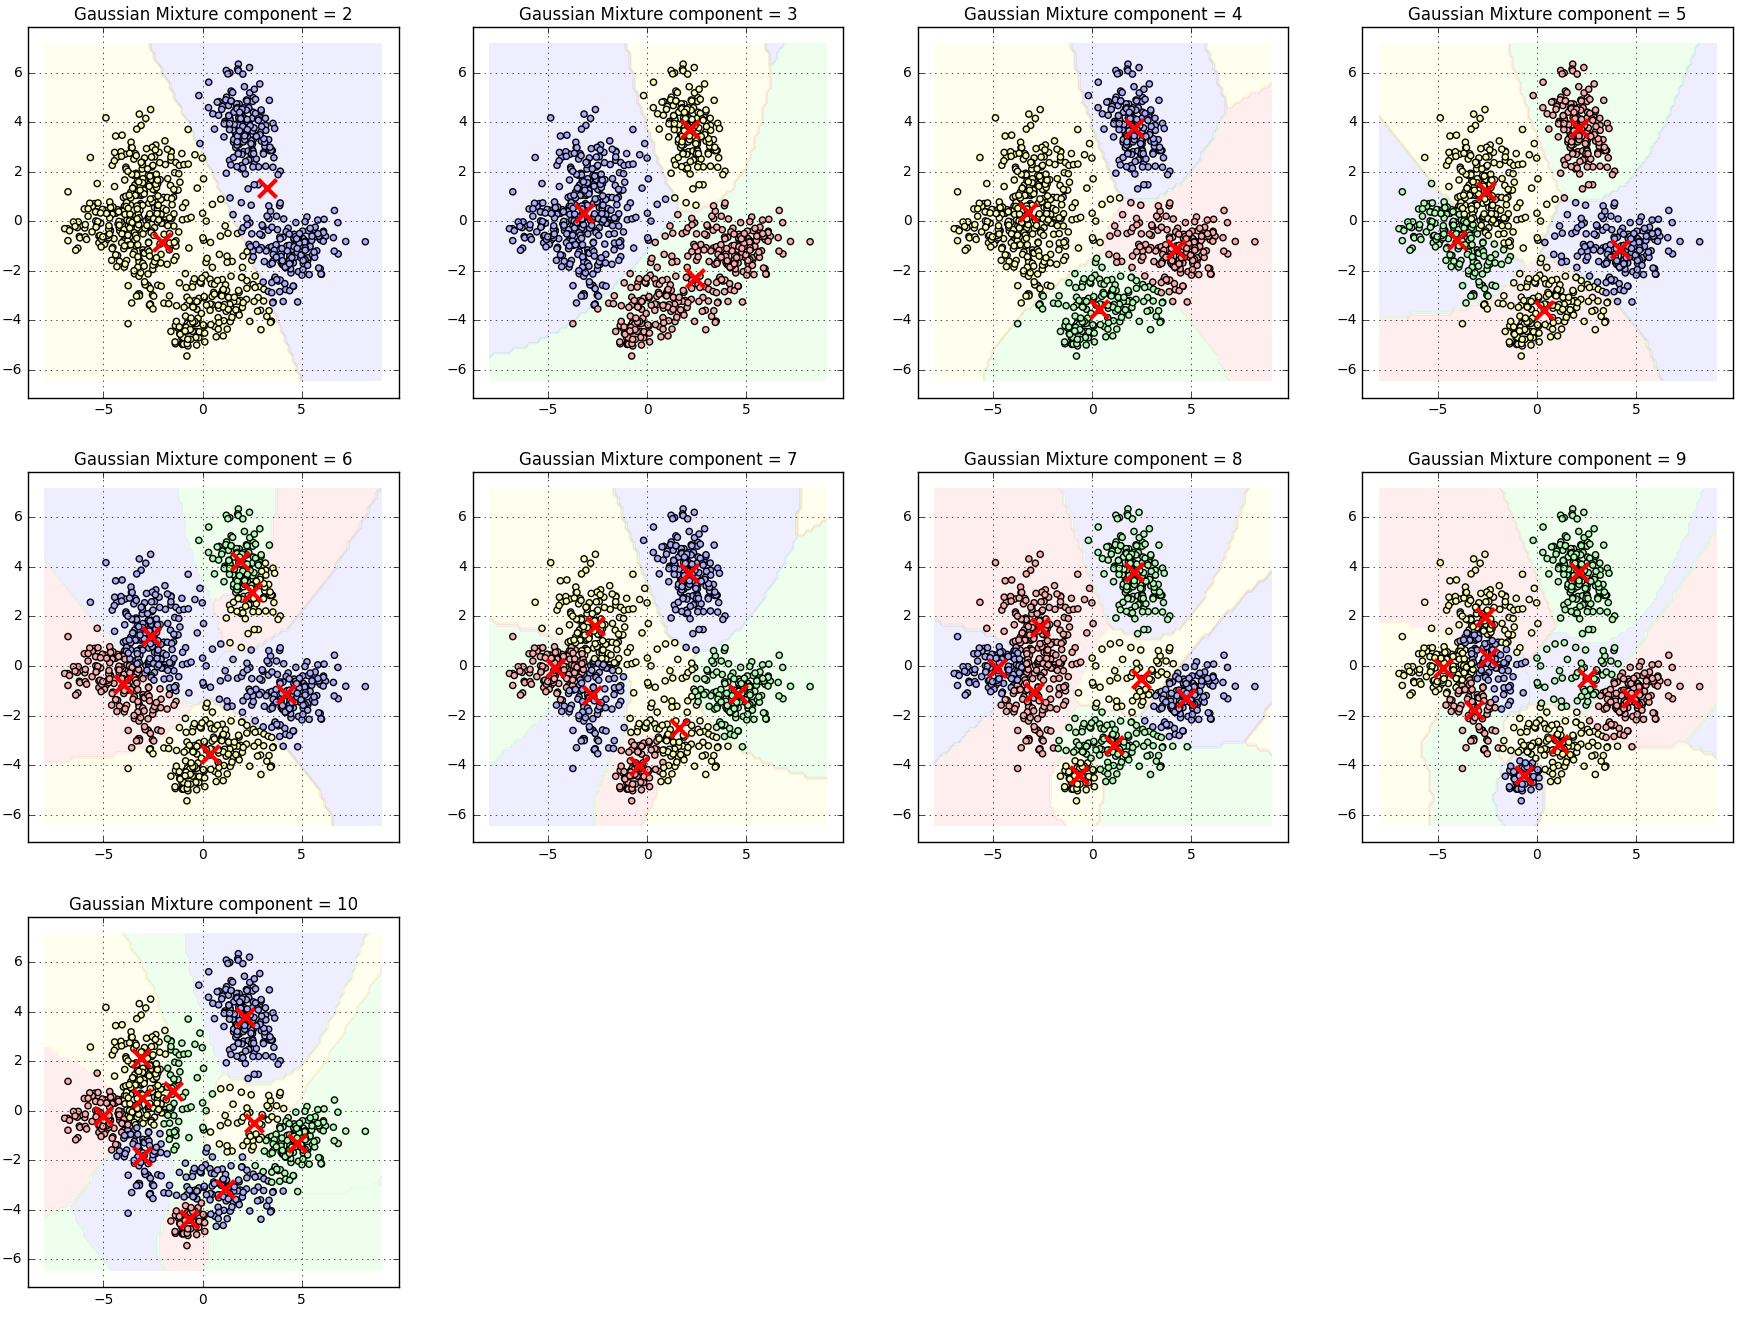
\includegraphics[scale=0.28]{3}
\end{center}
Here the result of clissified our data with GMM from 2 to 10 cluster.
 \\

\begin{figure}[h]
\centering
\begin{subtable}[h]{0.45\textwidth}
	 \begin{tabular}{|r | r | r | r|}
\hline
   K &   Normalized mutual &   Homogeneity &   Purity \\
\hline
   2 &            0.499168 &      0.321238 & 0.400666 \\
   3 &            0.669425 &      0.541329 & 0.592675 \\
   4 &            0.696318 &      0.630653 & 0.72475  \\
   5 &            0.695807 &      0.695294 & 0.847947 \\
   6 &            0.694674 &      0.720843 & 0.846837 \\
   7 &            0.692433 &      0.748394 & 0.849057 \\
   8 &            0.651789 &      0.726634 & 0.834628 \\
   9 &            0.674586 &      0.771993 & 0.851276 \\
  10 &            0.640276 &      0.751036 & 0.804661 \\
\hline

\end{tabular}
\end{subtable}
\begin{subfigure}[h]{0.45\textwidth}
 \centering

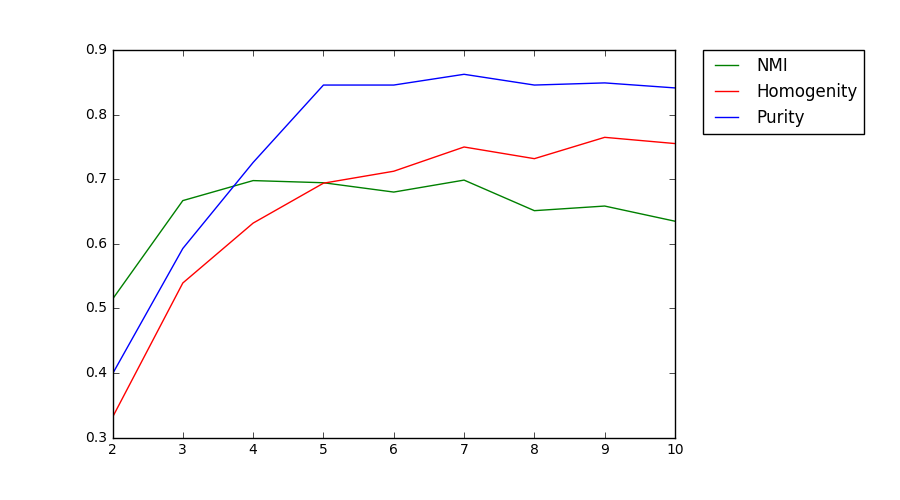
\includegraphics[scale=0.35]{4}

\end{subfigure}
\end{figure}
To compute purity , each cluster is assigned to the class which is most frequent in the cluster, and then the accuracy of this assignment is measured by counting the number of correctly assigned documents and dividing by $N$. This can gives a measure of the quality of the cluster.
 
 
\end{document}